\documentclass[runningheads]{llncs}

\usepackage{float}
\usepackage{tabularx}
\usepackage{siunitx}
\usepackage[a4paper, total={6in, 8in}]{geometry}
\usepackage[utf8]{inputenc}
\usepackage[english, romanian]{babel}
\usepackage[hidelinks]{hyperref}
\usepackage{indentfirst}
\usepackage[siunitx, RPvoltages]{circuitikz}
\usepackage{fancyhdr}
\usepackage{xspace}
\usepackage{amssymb}
\usepackage{layout}
\usepackage{lastpage}
\usepackage{titling}
\usepackage{leftidx}
\usepackage{array}
\usepackage{enumitem}
\usepackage{titletoc,tocloft}
\usepackage{xcolor}
\usepackage{amsmath}
\usepackage{nicefrac}
\usepackage{mathtools}
\usepackage{graphicx}

\begin{document}

\title{\textbf{Tema 1 - Proiectarea Algoritmilor}}

\author{Bogdan Alexandra-Lăcrămioara, 325CD}


\maketitle




\keywords{Divide et Impera \and MinMax \and Greedy \and Egyptian Fraction \and Programare dinamică \and Cutting a rod   \and Backtracking \and Fazan}


\section{Divide et Impera - Problema MinMax}


\subsection{Enunț}


Se citeste n, apoi n numere intregi.\newline
Calculaţi valoarea minimă minim și valoarea maximă maxim a celor n numere date.

\newline

\subsection{Date de intrare}

Fişierul de intrare "minmax.in" conţine pe prima linie numărul n si pe a doua linie n numere naturale separate prin spaţii\newline

\subsection{Date de ieșire }
Fişierul de ieşire "minmax.out" va conţine pe prima linie cele două numere, minim şi maxim, separate printr-un singur spaţiu.
\subsection{Input}
 8\newline
 10 23 5 7 25 2 3 1 
 \newline
\subsection{Output}
1 25\newline
\subsection{Pseudocod}

\begin{center}
    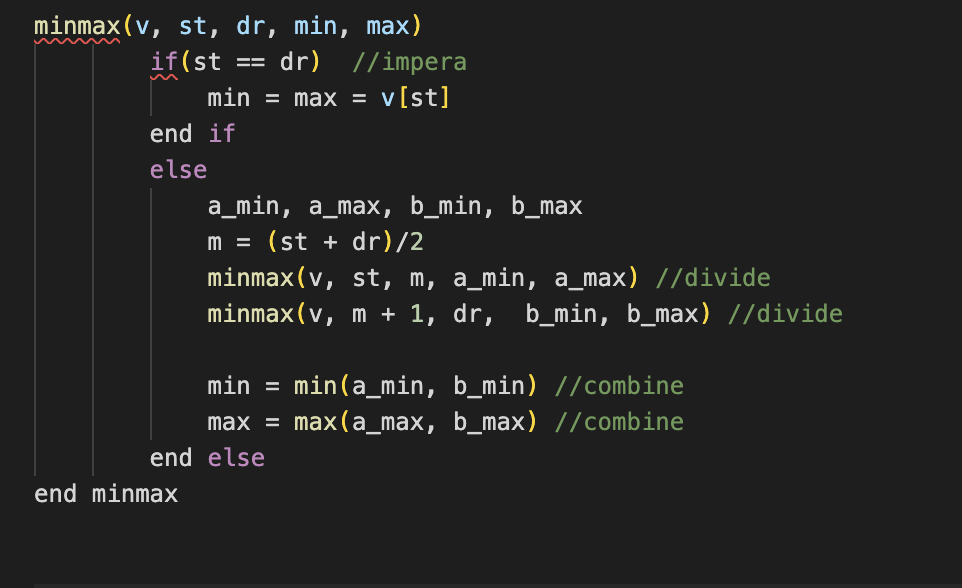
\includegraphics[scale=0.6]{p1.png}
\end{center}

\subsection{Descrierea soluției}
În ansamblu, algoritmul "minmax" folosește trei pași(impera, divide, combine) pentru a găsi valorile minime și maxime ale unui vector de numere întregi, împărțind intervalul în jumătăți, căutând valorile minime și maxime în mod recursiv și combinându-le în final pentru a obține rezultatele dorite. \newline
\begin{enumerate}

 \item Dacă indicele din stânga și cel din dreapta sunt egale (impera), atunci min și max vor fi egale cu valoarea vectorului de la acel indice.
\item În caz contrar (împarte):\newline
- Se calculează mijlocul intervalului (m = (st + dr) / 2).\newline
- Se apelează recursiv funcția minmax pentru jumătatea din stânga a intervalului și jumătatea din dreapta a intervalului.\newline
- Se obțin valorile minime și maxime pentru cele două jumătăți (a\_min, a\_max, b\_min, b\_max).\newline
\item Se combină valorile (combine):\newline
- Minimul va fi minimul dintre a\_min și b\_min.\newline
- Maximul va fi maximul dintre a\_max și b\_max.\newline
\item Se returnează valorile min și max.
 \end{enumerate}
În concluzie, algoritmul "minmax" împarte intervalul de căutare în jumătăți și calculează valorile minime și maxime pentru fiecare jumătate în mod recursiv, iar apoi combină valorile obținute pentru a obține valorile minime și maxime finale ale întregului interval.\newline
Algoritmul prezentat folosește o metodă top-down.
\subsection{Rularea pas cu pas a algoritmului pe inputul dat: 
}
\begin{center}
    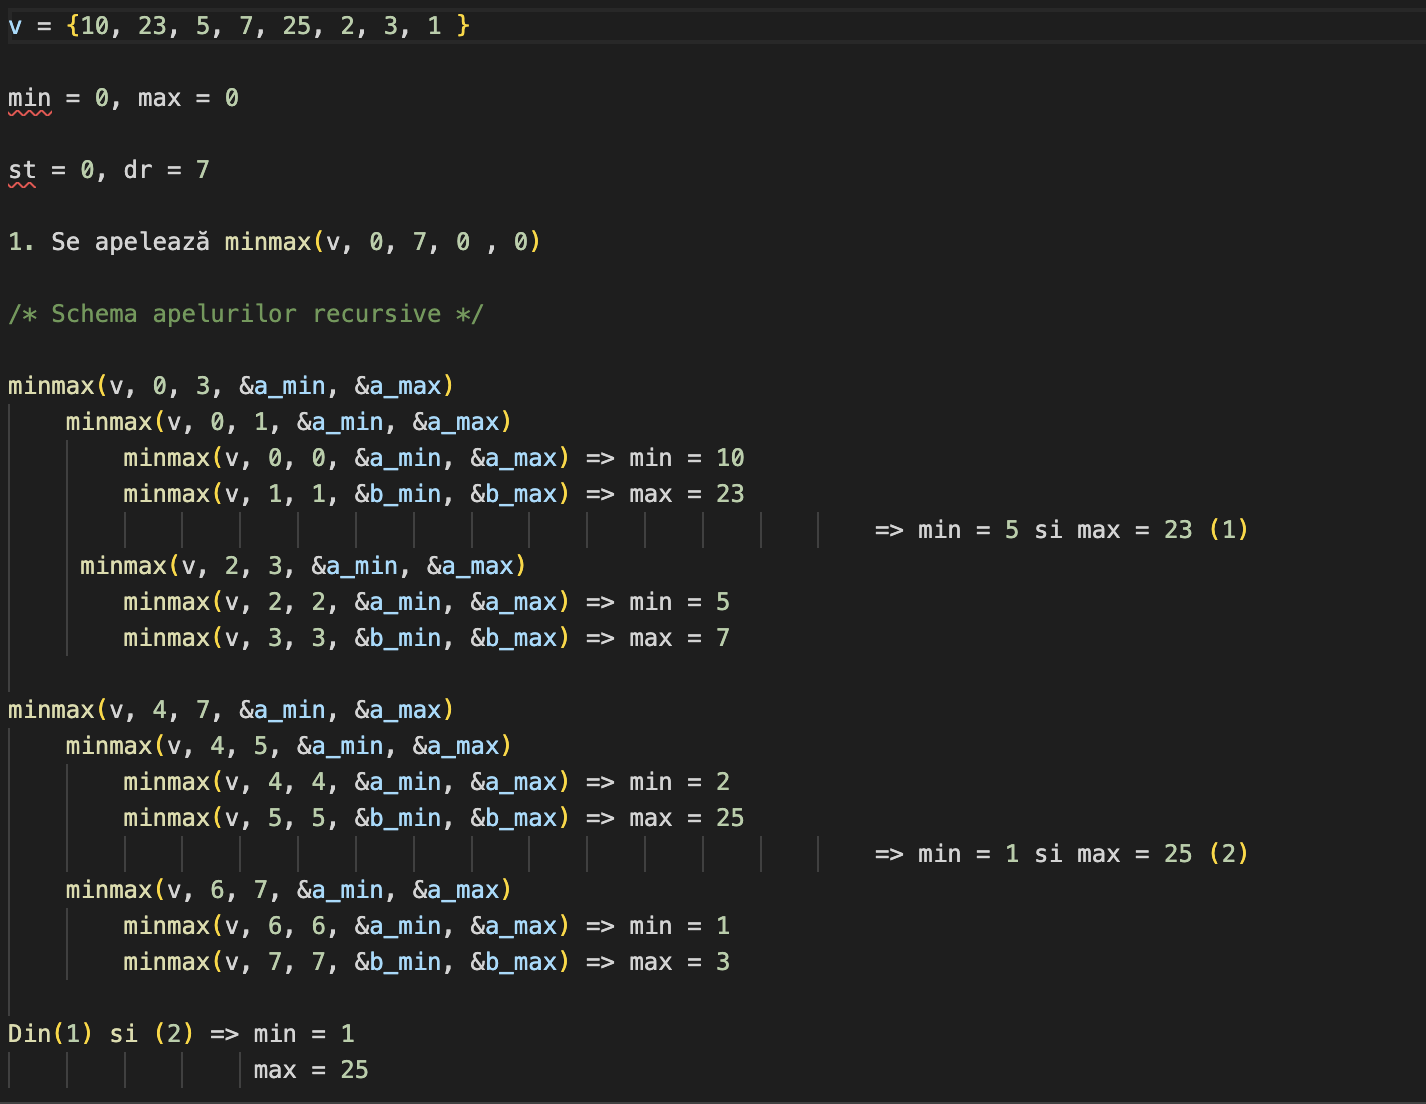
\includegraphics[scale=0.6]{p5.png}
\end{center}

Explicație:\newline

\begin{enumerate}
\item La început, apelăm funcția minmax cu vectorul v, și intervalul [0, 7], și inițializăm valorile pentru min și max cu 0.
\item Verificăm dacă st (începutul intervalului) este egal cu dr (sfârșitul intervalului). În acest caz, acestea nu sunt egale, așa că trecem la ramura else.
\item Calculăm mijlocul intervalului, folosind formula m = (st + dr) / 2, care în acest caz devine m = (0 + 7) / 2 = 3.
\item Facem două apeluri recursive ale funcției minmax pentru a calcula valorile minime și maxime ale vectorului v în două subintervale, [0, 3] și [4, 7].
\item Pentru subintervalul [0, 3], facem un alt apel recursiv al funcției minmax pentru a calcula valorile minime și maxime. Pentru [0, 1], găsim min = 5 și max = 23 prin apelurile recursive. Pentru [2, 3], găsim min = 5 și max = 7 prin apelurile recursive.
\item Pentru subintervalul [4, 7], facem un alt apel recursiv al funcției minmax pentru a calcula valorile minime și maxime. Pentru [4, 5], găsim min = 2 și max = 25 prin apelurile recursive. Pentru [6, 7], găsim min = 1 și max = 3 prin apelurile recursive.
\item La final, combinăm valorile minime și maxime calculate pentru cele două subintervale, obținând min = 1 și max = 25 ca valorile minime și maxime ale vectorului v în intervalul [0, 7].
\end{enumerate}

\subsection{Complexitate}

* { \bfseries Complexitate temporală:} O(n) \newline
\begin{center}
    
- Se deduce din recurența T(n) = \newline

 - T\left(\left\lfloor\frac{n}{2}\right\rfloor\right) + T\left(\left\lceil\frac{n}{2}\right\rceil\right) + 2 & \text{, pentru } n > 2 \\
 - 1 & \text{, pentru } n = 2 \\
 - 0 & \text{, pentru } n = 1 \\

\end{center}

* {\bfseries Complexitate spațială:} O(log(n)) \newline


\section{Greedy - Egyptian Fraction}


\subsection{Enunț}



Dat fiind un număr pozitiv rațional în formă de fracție proprie de forma unde a și b sunt numere întregi pozitive și cel mai mare divizor comun al lor este 1, problema fracțiilor egiptene constă în a găsi o serie finită de fracții 		unitare \newline

    
\begin{align*}
\sum_{i=1}^{n} \frac{1}{x_i}
\end{align*}



,unde xi sunt numere întregi pozitive, astfel încât suma acestor fracții să fie egală cu a/b.
\newline

\subsection{Date de intrare}
Programul citește din fișierul „ef.in”, pe prima linie, numărul a, iar 					numărul  b.\newline
\subsection{Date de ieșire}
Programul va afișa în fișierul „ef.out”, reprezentarea Egyptian Fraction a 				numărului de forma a/b.\newline

\subsection{Input}
6 14 \newline
\subsection{Output}

Egyptian Fraction representation of 6/14 is 1/3 + 1/11 + 1/231\newline

\subsection{Pseudocod}

\begin{center}
    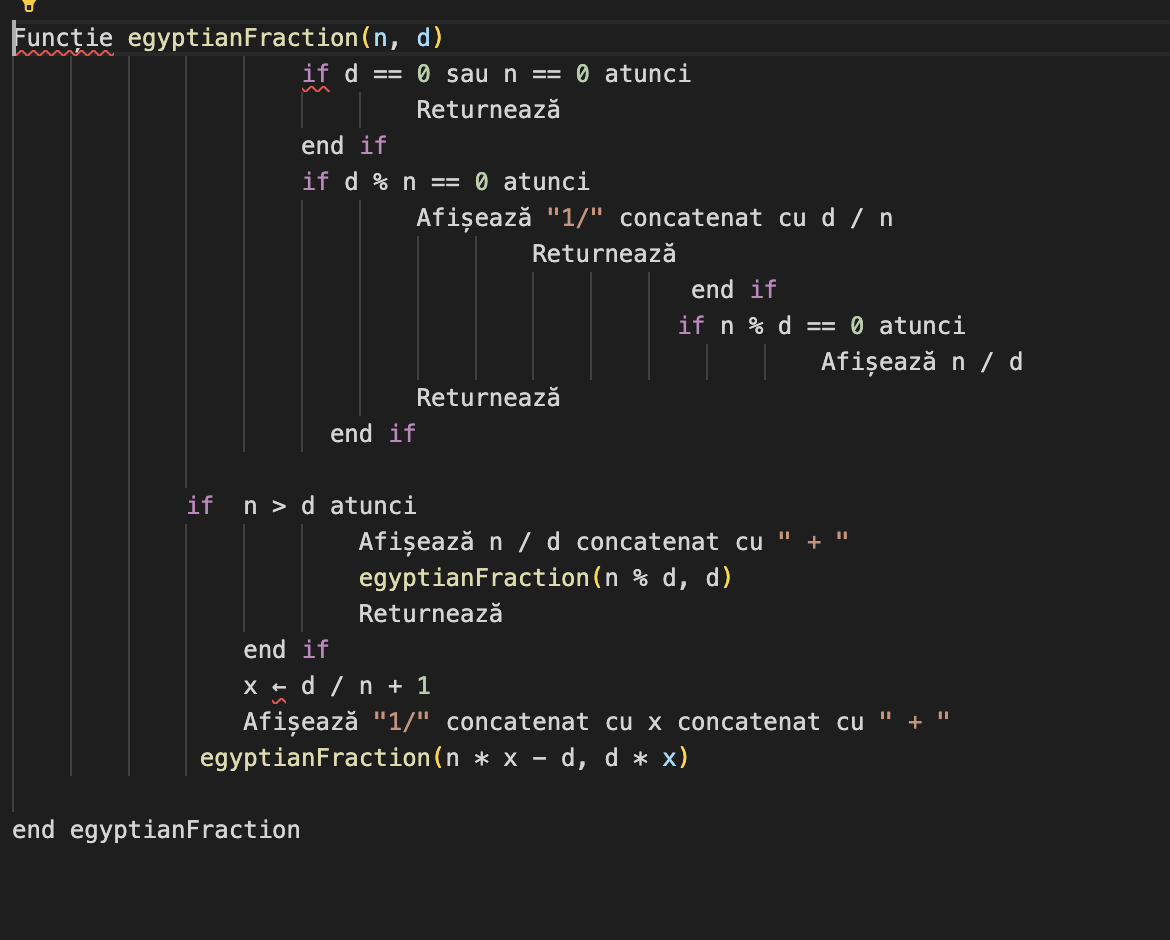
\includegraphics[scale=0.6]{p2.png}
\end{center}

\subsection{Descrierea soluției}

Definiție:
\begin{center}
    Fracție egipteană: Fracția egipteană, cunoscută și sub numele de fracție 					unitară, reprezintă o fracție cu numărătorul 1 si cu un numitor pozitiv, care 				este descompusă într-o sumă de fracții cu numărătorii 1 si cu numitori 					distincți si pozitivi.

\end{center}

\begin{enumerate}
\item \textbf{Pasul 1: Verificare d si n.} \
Algoritmul începe prin a verifica dacă $d$ este egal cu 0 sau $n$ este egal cu 0. Dacă una dintre aceste condiții este îndeplinită, algoritmul se oprește și nu afișează nimic, deoarece nu putem calcula fracții în care numitorul este 0 și nu avem nevoie de fracții egiptene pentru numărul 0.

\item \textbf{Pasul 2: Fracție unitară.} \\
Dacă $n/d$ poate fi exprimată ca o fracție unitară (adică $d$ este divizibil cu $n$), atunci algoritmul va afișa "1/" urmat de câtul dintre $d$ și $n$ și se va opri. Acest lucru se face pentru a simplifica fracția, deoarece o fracție unitară este deja o fracție egipteană.

\item \textbf{Pasul 3: Fracție întreagă.} \\
Dacă $n/d$ poate fi exprimată ca un număr întreg (adică $n$ este divizibil cu $d$), atunci algoritmul va afișa numărul întreg $n/d$ și se va opri. Acest lucru se face pentru a afișa direct rezultatul ca un număr întreg, deoarece nu este necesar să îl exprimăm ca fracție egipteană dacă este deja un număr întreg.

\item \textbf{Pasul 4: n mai mare ca d.} \\
Dacă $n$ este mai mare decât $d$, atunci algoritmul va afișa câtul dintre $n$ și $d$, urmat de "+", și apoi va apela funcția recursiv cu $n\%d$ și $d$, adică cu restul împărțirii lui $n$ la $d$ și cu $d$. Acest pas se repetă până când $n$ devine mai mic sau egal cu $d$. Acesta este procesul de descompunere a fracției în fracții egiptene, unde afișăm câtul și restul împărțirii, și continuăm acest proces până când restul devine mai mic sau egal cu numitorul.

\item \textbf{Pasul 5: n mai mic ca d.} \\
În cazul în care $n$ este mai mic decât $d$, atunci algoritmul va calcula $x = \frac{d}{n} + 1$ și va afișa "1/" urmat de $x$ și "+". Apoi, va apela funcția recursiv cu $nx-d$ și $dx$. Acest pas se repetă până când $n$ devine mai mic sau egal cu $d$. Acesta este procesul de descompunere a fracției în fracții egiptene, unde înlocuim
\item \textbf{Pasul 6: Returneaza rultatul} \\În final, funcția va returna rezultatul calculat, care va fi o 							concatenare a fracțiilor egiptene obținute prin pașii anteriori.
\end{enumerate}
			
\subsection{Rularea pas cu pas a algoritmului pe inputul dat:
}

Pentru inputul 6/14, algoritmul va fi rulat astfel:\newline

\begin{enumerate}
\item n = 6, d = 14
\item d \text{\%} n = 14 \text{\%} 6 = 2 , care nu este egal cu 0, deci se trece la următoarea condiție
\item n \text{\%} d = 6 \text{\%} 14 = 6, care nu este egal cu 0, deci se trece la următoarea condiție
\item Verifiare dacă n mai mare ca d. 6 mai mare ca 14? Nu, deci se trece la următoarea condiție
\item x = d / n + 1 = 14 / 6 + 1 = 2 + 1 = 3
\item Se afișează "1/3 + "
\item Se apelează recursiv egyptianFraction(n * x - d, d * x), adică egyptianFraction(6 * 3 - 14, 14 * 3)
\end{enumerate}

			Pasul recursiv:

\begin{enumerate}
    \item n = 6 * 3 - 14 = 4, d = 14 * 3 = 42
\item d\text{\%} n = 42 \text{\%} 8 = 2, care nu este egal cu 0, deci se trece la următoarea condiție
\item n \text{\%} d = 8 \text{\%} 42 = 8, care nu este egal cu 0, deci se trece la următoarea condiție
\item Verifiare dacă n mai mare ca d. 8 mai mare ca 42? Nu, deci se trece la următoarea condiție
\item x = d / n + 1 = 42 / 4 + 1 = 10 + 1 = 11
\item Se afișează "1/11 + "
\item Se apelează recursiv egyptianFraction(n * x - d, d * x), adică egyptianFraction(4 * 11 - 42, 42 * 11)
\end{enumerate}

			Pasul recursiv:
\begin{enumerate}
    \item n = 4 * 11 - 42 = 2, d = 42 * 11 = 462
\item d \text{\%} n = 294 \text{\%} 14 = 0, deci se realizează următoarele:
\item Se afișează "1/231"
\item Funcția se încheie, deoarece n și d sunt acum divizibile și se afișează fracția egipteană completă: "1/3 + 1/11 + 1/231".
\end{enumerate}
\subsection{Complexitate}

* { \bfseries Complexitate temporală:} O(n^2) \newline

* {\bfseries Complexitate spațială:} O(n) \newline
\subsection{Concluzii}
În concluzie, acest algoritm își are aplicabilitatea și în viața de zi cu zi, spre 				exemplu, atunci când trebuie să împărțim o cantitate limitată de resurse între 				mai multe persoane în mod echitabil. 



\section{Programare dinamică - Cutting a Rod}

\subsection{Enunț}

Dată fiind o bară de lungime n inch și un vector de prețuri care include 					prețurile tuturor bucăților de dimensiuni mai mici decât n, determinați 					valoarea maximă obținută prin tăierea barei și vânzarea bucăților obținute.

\subsection{Date de intrare}

* Datele se vor citi din fișierul „cr.in”\newline
*  O bară de lungime n, reprezentând lungimea inițială a barei de tăiat.\newline
* Un vector de valori v, unde v[i] reprezintă valoarea asociată bucății obținute prin tăierea barei la lungimea i ($1 \le $i \le n).


\subsection{Date de ieșire}
Programul va afișa în fișierul „ cr.out” valoarea maximă obținută.
\subsection{Input}
8\newline
1 8 6 9 10 17 20 20
			

\subsection{Output}
32
\subsection{Pseudocod}
\begin{center}
    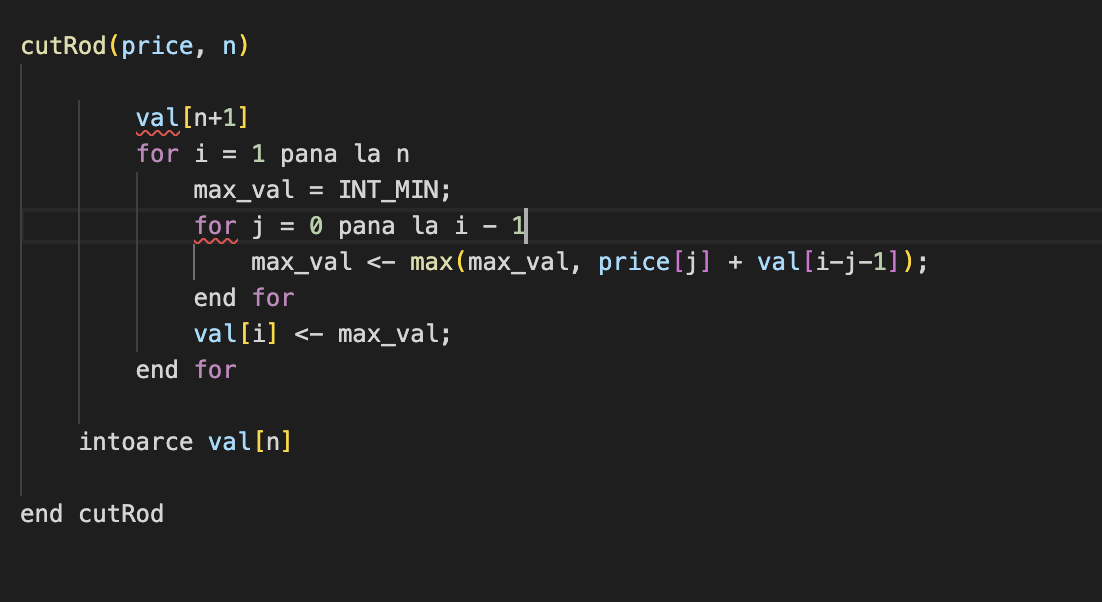
\includegraphics[scale=0.5]{p6.png}
\end{center}
\subsection{Descrierea soluției}
Algoritmul construiește o tabelă val de dimensiune n+1 pentru a stoca valorile maxime de profit obținute pentru lungimi de batonuri de la 1 la n.\newline

Descrierea pseudocodului: \newline
\begin{enumerate}
    \item Se inițializează val[0] cu 0, deoarece nu avem nicio lungime de bară disponibilă și, implicit, niciun profit.
    \item Se utilizează două bucle for pentru a itera prin toate lungimile posibile de la 1 la n. Prima buclă (i) reprezintă lungimea barei, iar a doua buclă (j) reprezintă toate posibilele tăieri ale acesteia, de lungime i.
    \item Pentru fiecare lungime i, se inițializează valoarea maximă cu o valoare minimă posibilă  pentru a urmări maximul de profit posibil pentru acea lungime.
\item Se iterează prin toate tăierile posibile ale barei de lungime i folosind bucla j, și se actualizează valoarea maximă cu suma dintre prețul tăierii curente (price[j]) și valoarea maximă de profit obținută anterior pentru bara rămasă după tăiere (val[i-j-1]), unde i-j-1 reprezintă lungimea barei rămase după tăiere.
Se actualizează val[i] cu valoarea maximă de profit obținută pentru lungimea de baton i.
\item După ce am iterat prin toate lungimile posibile, val[n] va conține valoarea maximă de profit obținută pentru bara de lungime n, care este răspunsul final al problemei.
\end{enumerate}
\subsection{Rularea pas cu pas a algoritmului pe inputul dat:}
 \begin{enumerate}
     \item Inițializăm valoarea lui val[0] cu 0.\newline
     val[0] = 0;\newline
n = 8;\newline
price = {1, 8, 6, 9, 10, 17, 20, 20};\newline

\item Pentru fiecare lungime posibilă a tăieturii, calculăm cel mai mare preț pe care îl putem obține și stocăm rezultatul în val[i], începând cu i = 1 până la n.\newline
\begin{center}
    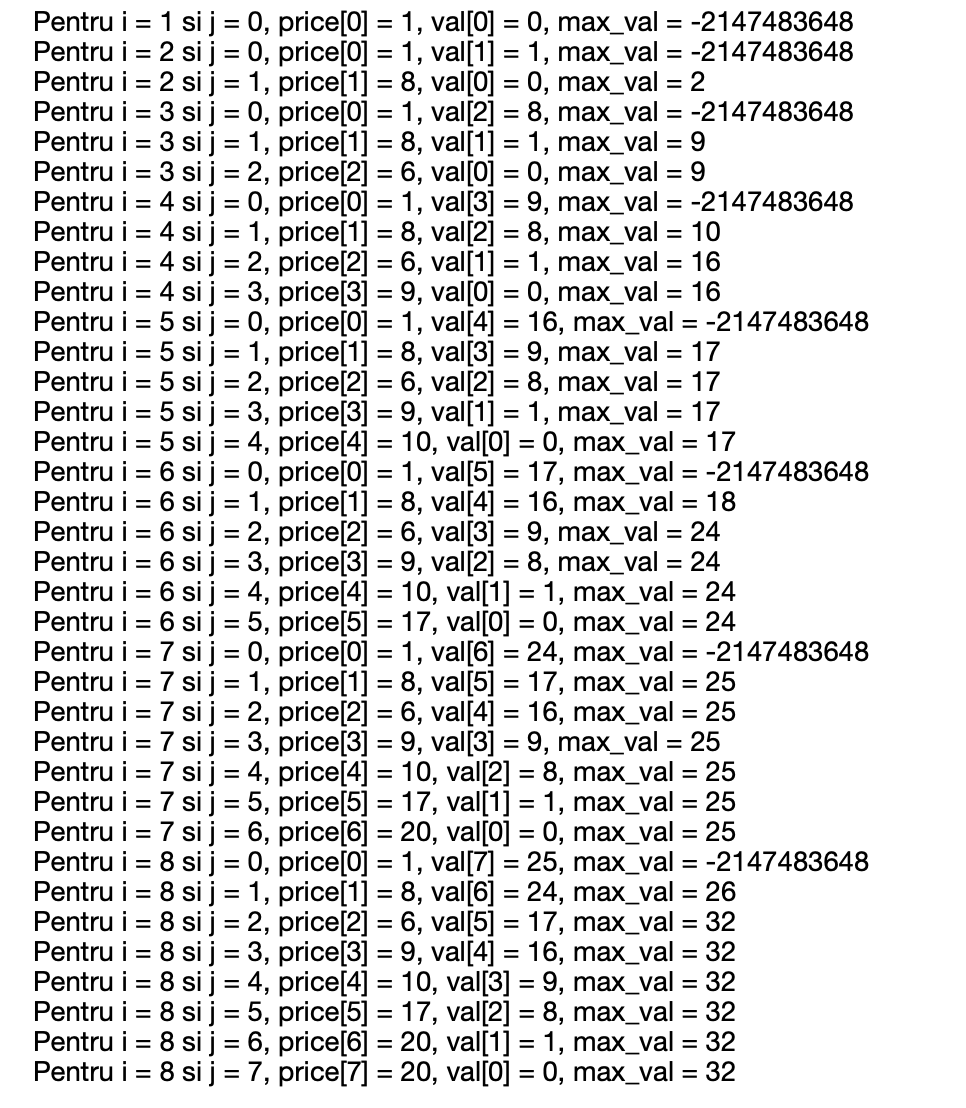
\includegraphics[scale=0.5]{1.png}
\end{center}
\item Se returneaza val[n].
 \end{enumerate}
 
\subsection{Complexitate}
* { \bfseries Complexitate temporală:} O(n*n)\newline 
  - deoarece utilizăm un singur vector val[n+1] pentru a stoca valorile calculate. Nu folosim alte structuri de date auxiliare de dimensiuni variabile în funcție de intrare, deci spațiul de memorie utilizat este proporțional cu dimensiunea de intrare n.\newline

* {\bfseries Complexitate spațială:} O(n),  deoarece utilizăm un singur vector val[n+1] pentru a stoca valorile calculate. Nu folosim alte structuri de date auxiliare de dimensiuni variabile în funcție de intrare, deci spațiul de memorie utilizat este proporțional cu dimensiunea de intrare n. \newline


\section{Backtracking - Fazan}

\subsection{Enunț}

Fiind date numerele naturale n, si m și apoi n cuvinte distincte cu cel mult 10 litere mici fiecare, să se afișeze toate secventele de câte m cuvinte dintre cele citite care să respecte condițiile jocului "fazan". 
\subsection{Date de intrare}

Se citesc din fisierul "fazan.in" numerele naturale n, și m, iar mai apoi, pe următoarea linie,  n cuvinte distincte.


\subsection{Date de ieșire}

Se afișează in fișierul "fazan.out" toate secvente de cate m cuvinte, care respectă regulile jocului "fazan" , fiecare secventă fiind urmată de un newline.

\subsection{Input}

8 3 \newline
paul alina asfalt nas ultim imagine nasture real 

\subsection{Output}

\begin{center}
paul ultim imagine\newline
alina nas asfalt \newline
alina nasture real \newline
nasture real alina \newline
real alina nas \newline
real alina nasture \newline
\end{center}
\subsection{Pseudocod}

\begin{center}
    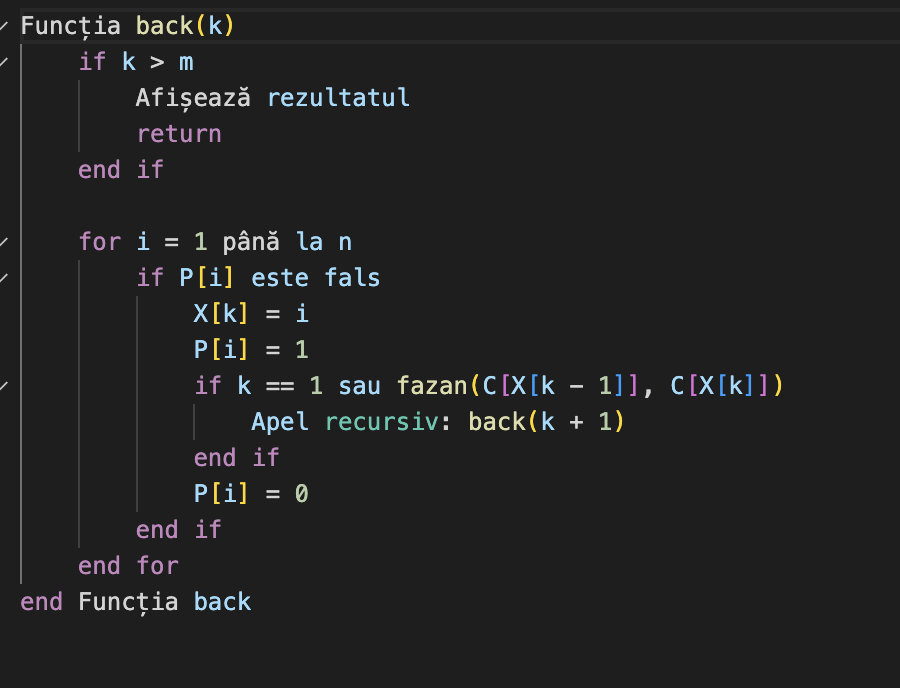
\includegraphics[scale=0.6]{p3.png}
\end{center}


\subsection{Descrierea soluției}

Funcția "back" folosește tehnica recursivă de backtracking pentru a genera toate permutările. Aceasta primește un parametru k, care reprezintă poziția elementului în permutare. Inițial, k este 1. Funcția parcurge toate elementele din setul de n elemente și verifică dacă elementul respectiv a fost deja folosit în permutare, prin intermediul vectorului P, unde P[i] este 1 dacă elementul i a fost folosit și 0 altfel. \newline

Dacă elementul nu a fost folosit, atunci acesta este adăugat în permutare la poziția k (X[k] = i), se marchează elementul ca fiind folosit (P[i] = 1) și se verifică dacă permutarea curentă este validă prin apelarea funcției "fazan" pentru ultimele două elemente adăugate în permutare și ultimele două elemente adăugate anterior în permutare. \neline

Dacă permutarea este validă și k este egal cu m (numărul de elemente din permutare), atunci se afișează permutarea. În caz contrar, se continuă să se genereze permutări, prin apelarea recursivă a funcției "back" cu parametrul k+1, pentru a adăuga următorul element în permutare.\newline

După terminarea funcției, toate permutările posibile au fost generate și afișate.\newline

Funcția "fazan" primește două șiruri de caractere, x și y, și verifică dacă ultimele două caractere din x sunt aceleași cu primele două caractere din y. Dacă da, funcția returnează 1, altfel returnează 0.
\subsection{Rularea pas cu pas a algoritmului pe inputul dat:}
\begin{center}
    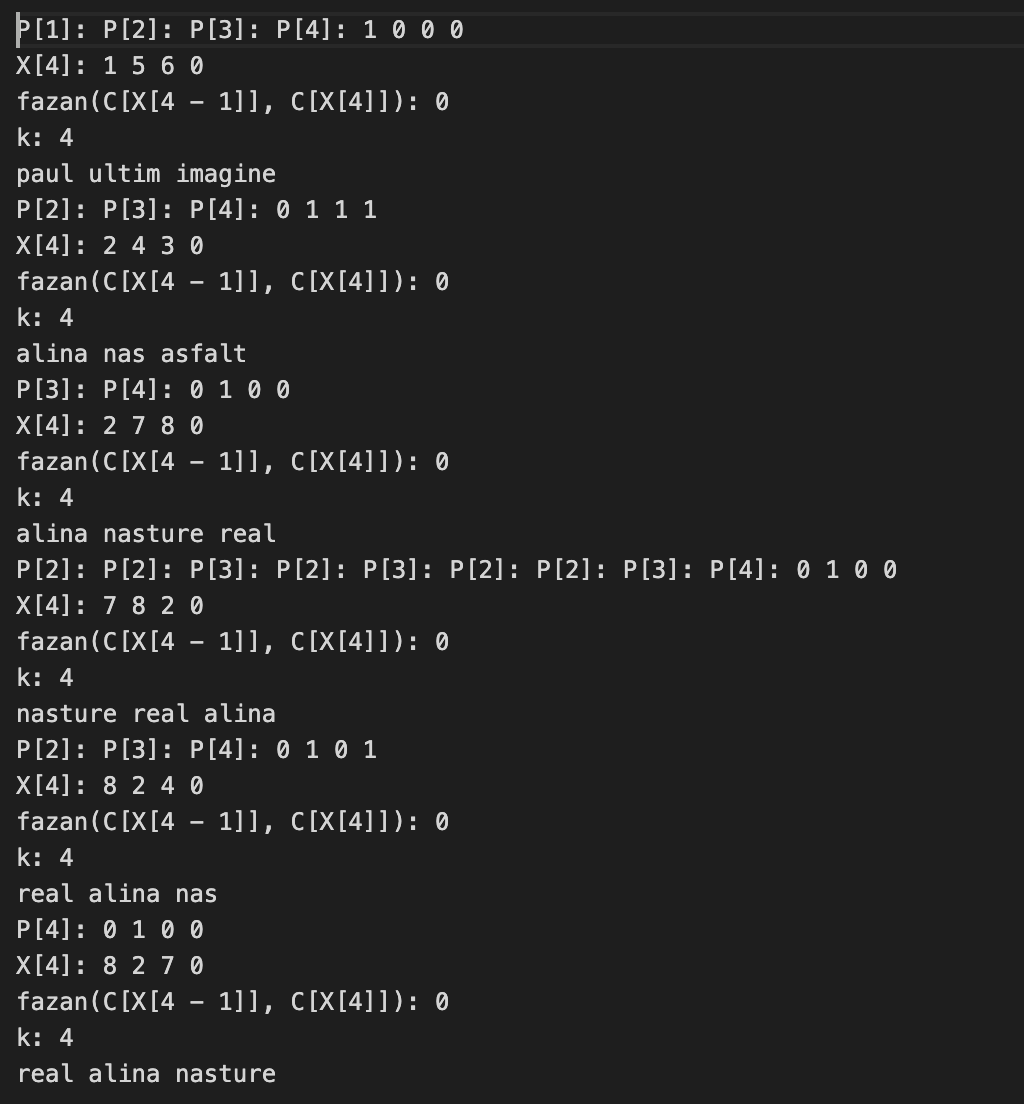
\includegraphics[scale=0.5]{p4.png}
\end{center}
\subsection{Complexitate}
* {\bfseries Complexitate temporală:}O(n!)\newline
  * { \bfseries Complexitate spațială:} O(n) \newline
  , unde n reprezintă numărul de cuvinte de intrare. 




\begin{thebibliography}{8}

\bibitem{ref_book}
"The Art of Computer Programming, Volume 1: Fundamental Algorithms" - Donald E. Knuth - Cap. Egyptian fractions (Section 1.2.8)
\bibitem{ref_url1}
https://www.pbinfo.ro/probleme/82/minmax , accesat ultima dată in 19.04.2023

\bibitem{ref_url2}
https:https://www.geeksforgeeks.org/greedy-algorithm-egyptian-fraction/ , accesat ultima dată in 19.04.2023

\bibitem{ref_url3}
https://www.geeksforgeeks.org/cutting-a-rod-dp-13/ , accesat ultima dată in 19.04.2023

\bibitem{ref_url4}
https://andrei.clubcisco.ro/2aa/diverse/Exercitii\%20complexitate\%20si\%20recursivitate.pdf, accesat ultima dată 19.04.2023


\bibitem{ref_url5}
https://info.mcip.ro/?cap=Backtracking\&prob=818 , accesat ultima dată 20.04.2023

\bibitem{ref_url6}
https://www.tutorialspoint.com/design\_and\_analysis\_of\_algorithms/design\_and\_analysis\_of\_algorithms\_max\_min\_problem.htm , accesat ultima dată 20.04.2023


\end{thebibliography}
\end{document}

